\chapter{Development}\label{ch:development}

\section{Digit classifier}\label{sec:digitclass}
Taking advantage of the convolutional neural networks (CNN) impressive performance in classification tasks, we have built a real-time digit classifier which captures images from any video stream, applies the necessary preprocessing and displays the predicted digit.

These are the major challenges that have been overcome during the development of the application:
\begin{itemize}
	\item Creating a dataset with images that resemble the ones found in the real world.
	\item Understanding how the CNNs work.
	\item Building a benchmark to evaluate the performance of the CNNs.
	\item Finding the optimal CNN model: architecture and learning process.
	\item Developing a GUI for the application.
\end{itemize}
\subsection{Datasets}\label{subsec:datasets}
MNIST database of handwritten digits is the starting point for the digit classifier. As it has been mentioned before \ref{sec:MNIST}, this database contains 60000 samples for training and 10000 samples for testing. Nevertheless, these large datasets may not be enough for our application, because they represent an \textit{ideal} situation.

\subsubsection{Edge detection}
The first problem with MNIST database is that the grayscale images that it contains share similar intensity levels: a white digit over a black background. In real world, the digits can be found written in several colors over different backgrounds and the datasets must resemble every possible combination. In order to achieve that generalization, an edge detection has been applied to the dataset. The resultant images are less dependent from the intensity values of the original ones, forcing the neural network to focus in the shape of the digits to classify them.

According to the study carried out by Nuria Oyaga \footnote{\url{http://jderobot.org/Noyaga-tfg\#Testing\_Neural\_Network}}, the edge detection algorithm that leads to better results is the Sobel filter. This operator approximates the gradient of an image function \cite{sonka2014image}, convolving the image with the following kernels to detect horizontal and vertical edges, respectively:  
\begin{equation}
h_x = 
\begin{bmatrix}
1 & 2 & 1\\
0 & 0 & 0\\
-1 & -2 & -1
\end{bmatrix}
,\quad
h_y = 
\begin{bmatrix}
-1 & 0 & 1\\
-2 & 0 & 2\\
-1 & 0 & 1
\end{bmatrix}
\end{equation}
The absolute values of the resulting images, $x$ and $y$, are then added, obtaining the edge image.

\subsubsection{Data augmentation with Keras}
The second problem that has been detected with MNIST is that the images are noiseless and the digits are always centered with a scale and a rotation angle that are almost invariant. However, the digit classifier has to deal with noisy images that can be randomly scaled, translated and/or rotated. In order to get a database with images that look like the ones that our application is going to work with, the MNIST database must be augmented.

Two alternatives have been considered to solve this problem: real-time data augmentation provided by Keras and generating our own database. In this section, the first one is going to be described.

Thanks to Keras \textit{.ImageDataGenerator()} method, the MNIST dataset can be augmented in real-time during training. In order to cover most of the real cases, random rotation, translation and zooming were applied to generate new samples. In addition to that, a Sobel filtering was also applied through a user-defined function. The samples generated by the following code can be seen in the figure \ref{fig:aug_keras}.

\begin{lstlisting}
	if mode == "full":
		datagen = imkeras.ImageDataGenerator(
			zoom_range=0.2, rotation_range=20, width_shift_range=0.2, 
			height_shift_range=0.2, fill_mode='constant', cval=0,
			preprocessing_function=self.sobelEdges)
	elif mode == "edges":
		datagen = imkeras.ImageDataGenerator(
			preprocessing_function=self.sobelEdges)

generator = datagen.flow(x, y, batch\_size=batch\_size)
\end{lstlisting}

\begin{figure}
	\centering
	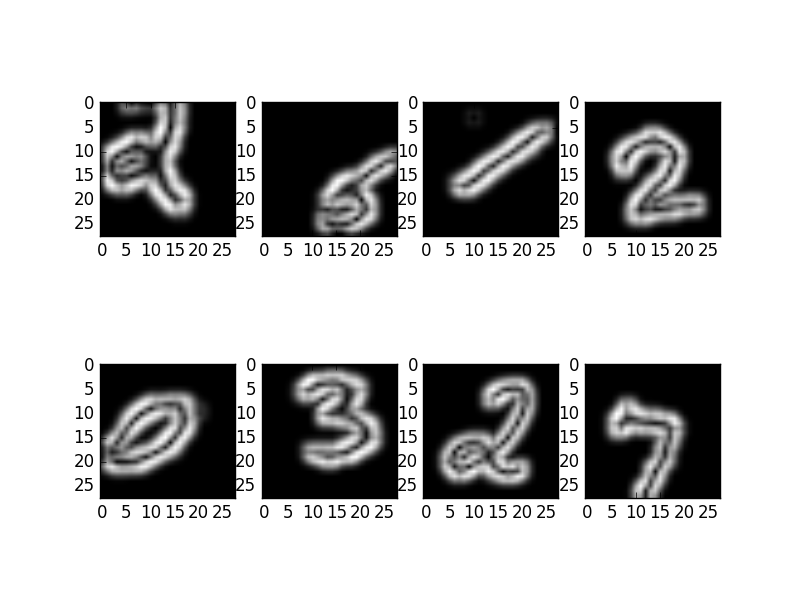
\includegraphics[width=12cm, keepaspectratio]{figures/aug_keras.png}
	\caption{Samples generated with Keras from MNIST database}
	\label{fig:aug_keras}
\end{figure}

Besides these transformations, it's also necessary to simulate the noise that will be present in real images. Keras generator doesn't support the addition of noise. For this purpose, Keras includes noise layers such as the GaussianNoise layer, which adds Gaussian noise with a standard deviation distribution defined by the user. It's important to note that Keras treat noise layers as regularization methods that are only active during training time to avoid over-fitting. In order to add noise to the generated samples, a GaussianNoise layer was established as the input layer of the model.
\subsubsection{Handmade augmented datasets}
\subsection{Classifier}\label{subsec:classifier}
\subsection{Benchmark}\label{subsec:bencharmk}
\subsection{Tuning the classifier}\label{subsec:tuning}
\subsection{\textit{digitclassifier.py}}\label{subsec:digitclassifier.py}
